\typeout{NT FILE chapter3.tex}
\chapter{Semantic Segmentation Models - Input data, algorithm and hyperparameters} \label{input_data_section}
\section{Input data} \label{input_data_sec}
The input data is one of the essential aspects of the model, characteristics such as image dimensions (in terms of pixels $W$x$H$), the number of bands ($D$) and even the number of images used for training, validation and test can influence the speed and performance of the chosen model.
\subsection{Labelled data} \label{labeled_data}
\paragraph{}
To be able to train a supervised \gls{DL} model, the availability of labelled data is essential in the process of training the model, this ground truth is the key in calculating the error and updating the weights of the model, until its loss and performance metric show good performance.
\paragraph{Thaw Slump Shape files}
The ground truth \gls{RTS} polygons were very kindly provided by Dr. Ingmar Nitze and the \gls{AWI}. These were collected across pre-defined sites in different locations at different timestamps and georeferenced for consistency and ease of use.

Two different types of shape files containing \gls{RTS} polygons were provided:
\begin{itemize}
    \item \textbf{Merged thaw slumps first iteration} Delineated by students and awaiting validation from Dr. Nitze, this type contains a total of $8,005$ features.
    \item \textbf{Merged thaw slumps validated} Delineated by students and validated by Dr. Nitze, this type contains a total of $1,203$ features.
\end{itemize}
\subsection{Sentinel-2 data} \label{sentinel2_section}
\paragraph{}
As mentioned in Section \ref{introduction}, the primary data source for this project will involve the use of Sentinel-2 satellite imagery. There are two product types available to users, Level 1-C Top Of Atmosphere reflectances and level 2-A Bottom Of Atmosphere reflectance images, both in cartographic geometry (\cite{sentinel2}). 

The latter is the one used in this project, as it is pre-processed to minimise atmospheric effects, leading to better normalisation across different regions.
There are 13 spectral bands available, from the \gls{VNIR} and \gls{NIR} all the way to the \gls{SWIR} (\cite{sentinel2}).

There are four 10 meter resolution bands: the three \gls{RGB} bands - Blue ($\approx$493 nm), Green ($\approx$560 nm), and Red (665 nm) plus a \gls{NIR} ($\approx$833 nm) band which is very important for vegetation detection. These are the ones initially used in this project.

In addition, there are six 20 metre bands: 4 narrow bands in the \gls{VNIR} vegetation red edge spectral-domain ($\approx$704 nm,$\approx$740 nm, $\approx$783 nm, and $\approx$865 nm) and 2 wider \gls{SWIR} bands ($\approx$1610 nm and $\approx$2190 nm) commonly used for snow/ice/cloud detection, or vegetation moisture assessments. Finally, two 60 metre bands mainly focused on cloud screening and atmospheric correction ($\approx$443 nm for aerosols and $\approx$945 nm for water vapour) and cirrus detection ($\approx$1374 nm).

\subsection{Sentinel-2 data collection} \label{rs_data_collection}
\paragraph{\gls{GEE} and JavaScript}
\paragraph{}
\gls{GEE} provides the ability of extracting satellite data using bespoke JavaScript queries through a Console \gls{UI} (shown in Figure \ref{gee_console_ui}, the Sentinel-2 data is available in the \gls{GEE} image collection with ID \textit{COPERNICUS/S2}.

    \begin{figure}[hbt!]
        \centering
        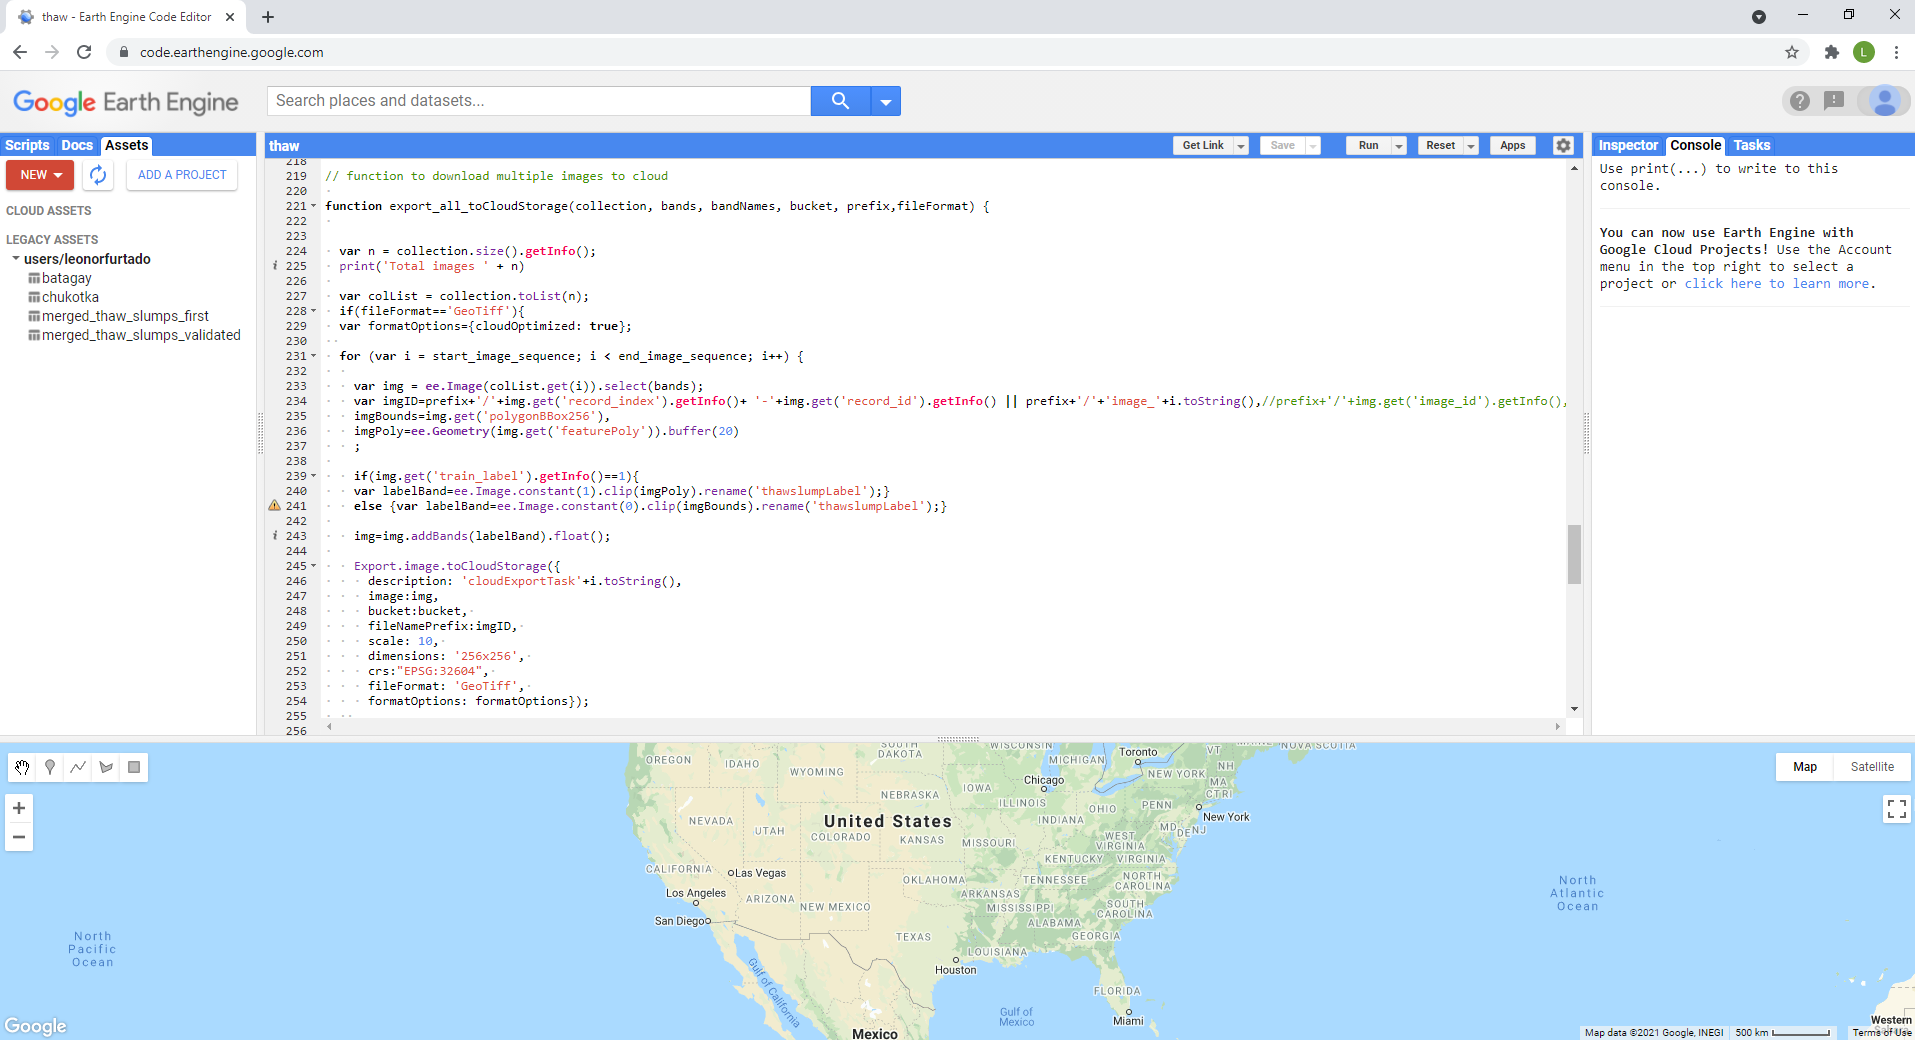
\includegraphics[width=0.85\textwidth]{gee_console_example.PNG}
        \caption{\gls{GEE} Console \gls{UI} showing a snippet of the bespoke JavaScript script}
        \label{gee_console_ui}
    \end{figure}

A bespoke JavaScript script was created that extracts satellite data for a fixed area and stores it in \gls{GCS}, this method of data collection will hereby be referred to as \textit{\gls{GEE} data}. This is an area of \SI{2.56}{\kilo\metre\squared}, so that the input size is close to 256x256 pixel representation, since for the highest resolution band one pixel represents a 10x10 \SI{}{\metre} area.

For positive label, when a (retrogressive) thaw slump is present in the area the data is extracted so that the \gls{RTS} polygons presented in section \ref{labeled_data} are at the centre of the image for the extraction.
For negative labels, control images are extracted based on \SI{2.56}{\kilo\metre\squared} squares centred around random points, that are checked for intersection with \gls{RTS} polygons and any overlapping random features are removed. 

This method has the limitation of introducing bias towards positive pixels always being in the centre of the image. This is a type of selection bias, as the subsample of images the model is being trained on does not represent the overall population of images, leading to poor generalisation of the model. For example, if the positive \gls{RTS} pixels are anywhere else but the centre of the image, the model would display poor performance
% , as will be shown and discussed in section \ref{}.

All images have the 10m resolution bands (\gls{RGB}, \gls{NIR} channels) plus thawslumpLabel.These correspond to the original Sentinel 2A bands B4, B3, B2 (\gls{RGB}),\gls{NIR} (B8) plus an additional thaw slump mask.This \gls{RTS} mask indicates pixels within thaw slump polygons, plus a 20 \SI{}{\metre} (approximately 2 pixels) edge buffer, with value 1 and all other pixels set as 0 in other parts of the image (in control images this band is all 0s).
Each satellite image has been collected to match the polygon image date as closely as possible, within a $+/-$ 2-week window. This range is wide as the images extracted exclude any images with cirrus and clouds. This dataset will be hereby referred to as \textit{\gls{GEE} data}.

Files are in GeoTiff format with float32 pixel values that have not been scaled, so are in raw format at this stage, these values returned by the \gls{GEE} API that can reach values of $10,000$ or more in some instances. This is the case as even though reflectances are typically percentage values between $0$ and $100$ (or $0$-$1$), these are often scaled by a certain factor (e.g. $1 e^4$) to be able to use integer values instead to save disk space. 

The \gls{CRS}, which associates numerical coordinates with a position on the Earth's surface, is defined by organisations such as the \gls{EPSG}.

The projections are identified through an authority:code format, where the authority is for example “\gls{EPSG}” and the code is a unique number for a given \gls{CRS}. For example, \gls{EPSG}:32604 was used for this project's data extraction for \gls{RTS}s located in Herschel Island.

This method of data collection came with its limitations, the \gls{GEE} \gls{UI} would crash for more than 30 images extracted at any one time and would freeze while extracting those images, taking hours at a time. This method wasn't automatable, which explains why the number of images collected is so low compared to the number of features in the polygons provided as ground truth.
\paragraph{\gls{GCS} and \gls{JP2} data}
\paragraph{}
To address both the bias and automation limitations of the \gls{GEE} method, downloading images directly from \gls{GCS} was explored latter in the project.

Sentinel-2 data is made free and available on \gls{GCP} by the European Commission and the European Space Agency(ESA) as part of the Google Public Cloud Data program. The data is made available in a \gls{GCS} public bucket (\textit{gs://gcp-public-data-sentinel-2}) in the \gls{JP2} format, it is stored as tiles of approximately \SI{100}{\kilo\metre\squared}, according to the Sentinel-2 tiling grid (based on the Military grid reference system) at a particular point in time, referred to as a \textit{granule} (\cite{sentinel2_gcp}).

This method involved downloading granules that contained sites used for the collection of the merged thaw slumps validated labelled data presented in section \ref{labeled_data} at the time the labels were delineated +/- $1$ month as a filter to guaranty low ($0-10\%$) cloud coverage, was applied.

The polygons were reprojected from \gls{EPSG}:$4326$ to the respective \gls{CRS} associated with each of the extracted tiles, data was then consolidated in a data cube containing the same 10 m resolution bands (\gls{RGB}, \gls{NIR} channels)  shown in Figure \ref{thaw_slump_img} after normalisation, plus the thaw slump mask shown in Figure \ref{thaw_slump_mask}. Dta was split using sliding windows of 64x64 pixels,after this any empty tiles, ones without any positive \gls{RTS} pixels and ones with unexpected reflectance patterns were discarded. This pre-processed input data was kindly provided by Adam Wickenden as part of Accenture's collaboration  with \gls{SEI} and \gls{AWI} and will be hereby referred to as \textit{\gls{JP2} data}.

\begin{figure}[hbt!]
    \begin{minipage}[c]{0.45\linewidth}
        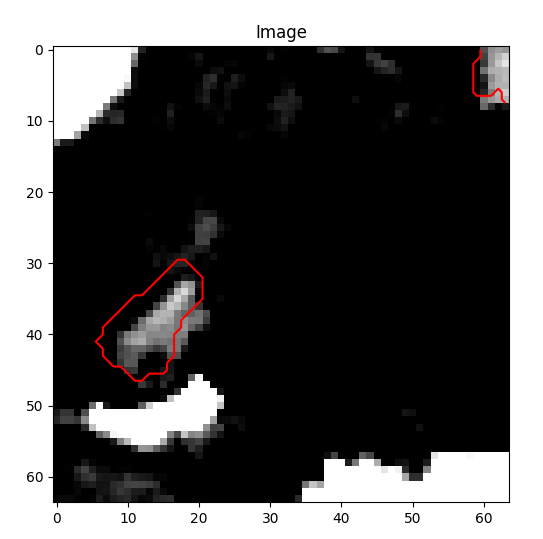
\includegraphics[width=\linewidth]{thaw_slump_z_score.PNG}
        \caption{Example of the \gls{RGB} channels normalised using z-score}
        \label{thaw_slump_img}        
        \end{minipage}
        \hfill
        \begin{minipage}[c]{0.45\linewidth}
        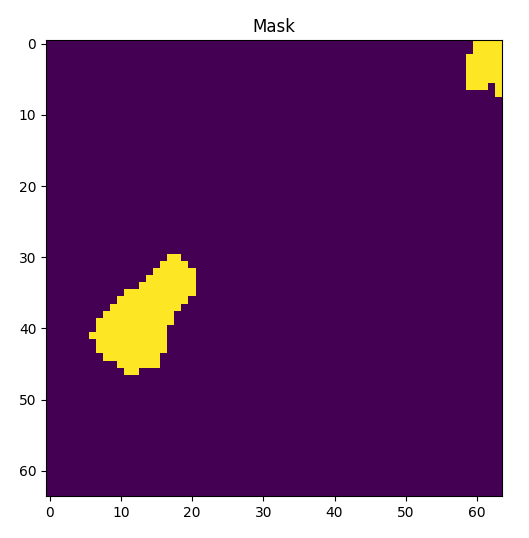
\includegraphics[width=\linewidth]{thaw_slump_mask_z_score.PNG}
        \caption{Example of a \gls{RTS} mask}
        \label{thaw_slump_mask}
    \end{minipage}
\end{figure}

\subsection{Data understanding and preparation} \label{dataprep}
\subsubsection{Scene classification labelled data}
\paragraph{}
The original \textit{\gls{GEE} data} collection method extracted a total of 313 scenes containing \gls{RTS} positive samples, and 311 control negative samples containing only background pixels. These were split into train and validation datasets with a $80$/$20$ proportion respectively. A stratified method was used to ensure class representation and avoidance of class imbalance in any one dataset. These datasets were used in the training of the initial scene classification model introduced:
\begin{table}[ht!] 
    \begin{center}
    \begin{tabular}{c|c|c}    
    \textbf{Dataset} & \textbf{Thaw Slump} & \textbf{Control} \\
    \hline
    Train 
    &  250
    & 249  \\
    \hline
    Validation 
    &  63
    & 62  \\
    \hline
    Total 
    &  313
    & 311  \\
    \hline
    \end{tabular}
    \end{center}
    \caption{Distribution of \gls{GEE} data for scene classification}\label{table_label_data_class}
\end{table}
\subsubsection{Pixel-wise classification labelled data}
\paragraph{}
In terms of pixel distribution in each image, there is an imbalance for semantic segmentation models, that are given proportionally more negative background pixels than positive \gls{RTS} pixels. 
Figure \ref{rts_pixel_dist} depicts the distribution of pixels with \gls{RTS} positive label in the \textit{\gls{GEE} data}, as it can be seen from the figure most images have less than 500 pixels of the positive class which is less than $1\%$ of a 256×256 pixel image.

    \begin{figure}[hbt!]
        \centering
        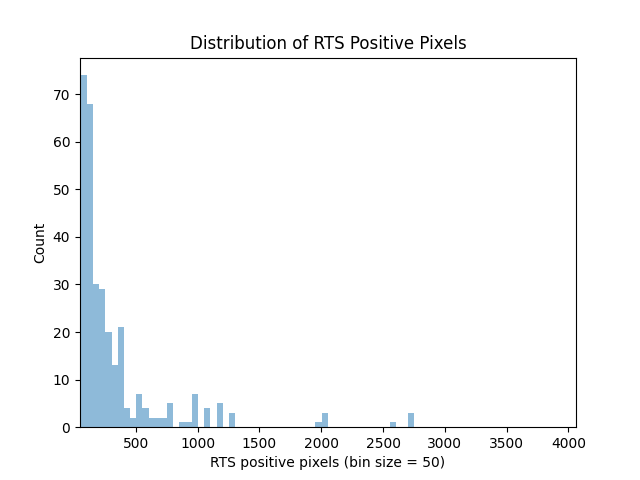
\includegraphics[width=0.55\textwidth]{Distribution of RTS Positive Pixels.png}
        \caption{Distribution of \gls{GEE} data \gls{RTS} positive pixels}
        \label{rts_pixel_dist}
    \end{figure}
    
To train the segmentation models, only the 313 images in the \textit{\gls{GEE} data} containing positive \gls{RTS} pixels were used for training, to avoid further imbalances in the model towards background negative pixels, for training the data was split as follows:
\begin{table}[ht!] 
    \begin{center}
    \begin{tabular}{c|c|c}     
    \textbf{Dataset} & \textbf{Thaw Slump} & \textbf{Percentage of total} \\
    \hline
    Train 
    & 250 & 80\% \\
    \hline
    Validation 
    &  47 & $\approx 15\%$  \\
    \hline
    Test 
    &  16 & $\approx 5\%$ \\
    \hline
    Total 
    &  313 & 100\% \\
    \hline
    \end{tabular}
    \caption{Train/ Validation/ Test split of samples for \gls{GEE} data} \label{table_label_data_gee}
    \end{center}
\end{table}

Later in the project the \textit{\gls{JP2} data} was introduced with a total of $585$ $64$x$64$ slices containing positive \gls{RTS} pixels that can be used for the supervised \gls{DL} model it's distribution is as follows:

\begin{table}[ht!] 
    \begin{center}
    \begin{tabular}{c|c|c}     
    \textbf{Dataset} & \textbf{Thaw Slump} & \textbf{Percentage of total} \\
    \hline
    Train 
    & 468 & 80\% \\
    \hline
    Validation 
    &  90 & $\approx 15\%$  \\
    \hline
    Test 
    &  27 & $\approx 5\%$ \\
    \hline
    Total 
    &  585 & 100\% \\
    \hline
    \end{tabular}
    \end{center}
    \caption{Train/Validation/Test split of samples for \gls{JP2} data} \label{table_label_data_jp2}
\end{table}

Figure \ref{jp2_rts_pixel_dist} depicts the distribution of pixels with \gls{RTS} positive label in the \textit{\gls{JP2} data} across different datasets, to attempt a stratified sampling method the random seed was changed until the distribution looked similar across the datasets.
% as it can be seen from Figure \ref{thaw_slump_mask} in section \ref{rs_data_collection}.

    \begin{figure}[hbt!]
        \centering
        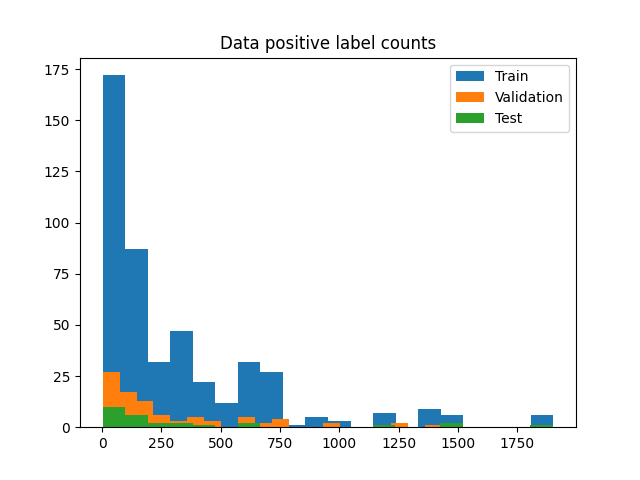
\includegraphics[width=0.75\textwidth]{jp2_rtscount_split.png}
        \caption{Distribution of \gls{JP2} data \gls{RTS} positive pixels across datasets}
        \label{jp2_rts_pixel_dist}
    \end{figure}
\section{Introduction to semantic segmentation models}
\paragraph{}
Given the literature on remote sensing \gls{DL} problems, along with the labelled \gls{RTS} data available in a mask format, where each pixel is labelled, it makes sense to make the focus of this project the semantic segmentation networks based on CNN models that were introduced in section \ref{seg_nets}.

These different architectures will be evaluated in experiments, as well as the architecture parameters, that is, Kernel sizes, stride, number of layers, number of filters etc. which nowadays are also considered "hyperparameters" that feed into the learning process described in section \ref{nn_hyperparameters}, since these were covered in section \ref{cnn_layers}.

To evaluate the success of the task at end in pixel-wise classification models in remote sensing, the ground truth is imputed as a mask of values, $1$ for thaw slump and $0$ for background. The other input is the satellite image itself. To bring the best out of the model architecture, this data needs to be pre-processed to be turned into the input that the network is expecting, usually in tensor form with values between $0$ and $1$.

The model architecture itself also plays an important part in the success of the model, its complexity/depth as well as the architecture parameters described above need to be adequate for the problem at hand.

In addition to this, the network hyperparameters also need to be defined before the training can start. After this is done, the training process can start where the model parameters i.e. weights are optimised so that the predictions of \gls{RTS} or no-\gls{RTS} performed by the model match the mask ground truth as closely as possible.

\subsection{Pre-processing of data} \label{data_preproc}
\subsubsection{Resizing images} \label{img_resize}
\paragraph{}
In segmentation models, the spatial size of the input tensor has an impact on the performance of the model. With lower dimension sizes a more complex architecture could be required (higher number of filters), however with  greater dimensions more training samples are likely to be needed.

So it is important to have input image dimensions ($W$ x $H$) that are adequate for the problem at hand, especially when the \gls{RTS} only covers a small area (a few pixels, since each pixel represents a 10 m x 10 m area.

There are a few ways of increasing the dimensions of an image through different interpolation strategies, some of them are:
    \begin{itemize}
        \item \textbf{Bilinear interpolation} mentioned before as one of the segmentation model upsampling strategies, it takes the weighted average of the $4$ nearest pixels for the new pixel value
        \item \textbf{Bicubic interpolation} similar to bilinear, but instead uses the  $4$x$4$ neighbourhood i.e. 16 pixels to calculate the new value, again weighted more on the closest pixels. 
        \item \textbf{Nearest neighbour} simply returns the value of the nearest pixel according to the interpolation coordinates.
    \end{itemize}
\subsubsection{Normalisation techniques} \label{img_norm}
\paragraph{}
Unlike natural images that have a known value between $0$ and $255$, remote sensing imagery depends highly on the scale of the reflectance values returned by the \gls{GEE} API varying widely and reaching values of over  $10,000$ in some instances, therefore the normalisation of input becomes quite important.

To feed input values into the \gls{NN} it is better to normalise them between $[0,1]$, this is particularly challenging in remote sensing imagery as the spectral data has a big variation of reflectance values across bands and images. 

A na\"ive approach of simply converting any pixel $x>10,000 =10,000$ and then dividing by $10,000$ was the first method attempted, given that most band's reflectance values go up to $10,000$ with a few outliers above $10,000$.

There have been a couple of strategies presented in a few remote sensing papers that could be possible solutions.

In other remote-sensing imagery normalisation the authors normalise the values per spectral band (\cite{8516352}) using in the interval $[0,1]$, others use the z-score to
approximate the distribution of pixel values of the input to a normal distribution (\cite{Zhong2017SatCNNSI}). 

They are both converted to spectral band-wise normalisation using the below definitions (\cite{BELENGUERPLOMER2021112468}):

\begin{equation} \label{eq_interval}
interval [0,1](x) = \frac{x}{max(b)}
\end{equation}

\begin{equation} \label{eq_z_score}
z-score(x) = \frac{x- \mu(b)}{\sigma(b)}
\end{equation}

where $x$ is any given pixel and $b$ is any given spectral band of the image.

\subsubsection{Data Augmentation} \label{img_aug}
\paragraph{}
Due to the biased data collection method described in section \ref{rs_data_collection}, making the \gls{RTS} positive pixels the centre of the training patch, it is essential to apply data augmentation techniques that will vary this feature of the training set, so that the model is not biased towards finding positive labelled pixels only at the centre of the image provided. 

For that purpose and also the general purpose of introducing noise in the model to make it more robust and less subject to overfitting due to the small sample size, the following data augmentation techniques are presented:

    \begin{itemize}
        \item \textbf{Random horizontal or vertical flipping} Randomly flips the image and mask horizontally or vertically.
        \item \textbf{Cropping} randomly crops the image and mask
        \item \textbf{Scaling} randomly rescales the image by shrinking it or stretching it keeping the same ratio, in this case a square image.
        \item \textbf{Blurring} different satellites resolution could introduce blurring, so it is important to introduce that to make the model more robust.
        \item \textbf{Shifting} shifts the coordinates of every pixel along the image axis, important to avoid that centred \gls{ROI} bias.
    \end{itemize}
\subsection{Preparing the data for modelling using Tensorflow} \label{tf_dataprep}
A bespoke script was created to code a data generator compatible with Tensorflow models there are a few steps in the model:

\begin{enumerate}
    \item Read GeoTiff file and convert it to tensor format
    \item Select the $m$ bands for $X$ and thaw slump label/mask for $y$
    \item Image normalisation technique applied
    \item Generates batches of data for training
\end{enumerate}
\subsection{\gls{DL} Learning process} \label{nn_hyperparameters}
\paragraph{}
To successfully train any \gls{NN}, there are a few key "ingredients" that are necessary to ensure any given model with its own architecture and parameters to enable it to accurately perform the task of matching its predictions with the ground-truth. These will be covered in this section:

\begin{enumerate}
    \item \textbf{Loss/cost function} that evaluates how well the model performs on any given task, where the goal is usually to minimise the loss.
    \item \textbf{Activation function} will define how the activation map is calculated after convolution and fully connected layers. These were covered in detail in section \ref{cnn_activation}, the ones most widely used in pixel-wise classification architectures in remote sensing are \gls{ReLU} and its variants.
    \item \textbf{Optimiser} responsible for updating the model parameters at each iteration to optimise the cost function. To learn the model parameters (\gls{a.k.a.} weights in a \gls{NN}) efficiently, essential hyperparameters that estimate the parameters need to be adjusted "manually" as depicted in Figure \ref{fig_hyperparameter}:
        \begin{enumerate}
            \item \textbf{Batch Size} determines the frequency of updates influencing convergence and generalisation.
            \item \textbf{Initialiser} a good initialisation can accelerate optimisation and enable convergence.
            \item \textbf{Regulariser} introduces noise to reduce overfitting.
            \item \textbf{Learning Rate} influences the optimisation’s convergence.
        \end{enumerate}
        
\end{enumerate}

    \begin{figure}[hbt!]
        \centering
        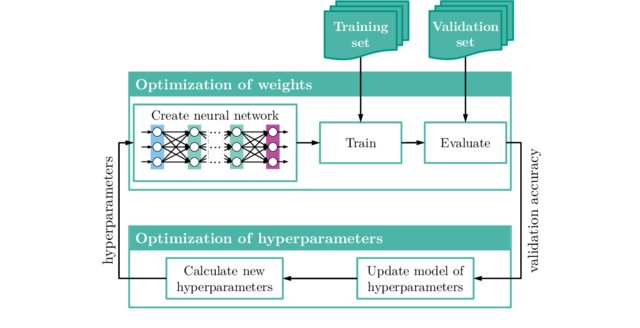
\includegraphics[width=0.75\textwidth]{flowchart_hyperparameter.jpg}
        \caption{NN hyperparameter optimization cycle (\cite{hyperparameter_fig})}
        \label{fig_hyperparameter}
    \end{figure}
\subsubsection{Loss function} \label{loss_functions}
The loss function is one of the essential components in the learning process of \gls{DL} models, since it enables the \gls{DL} algorithms to learn and optimise the objective through gradient descent. The loss function is responsible for ensuring that the mathematical representation of the objectives is accurate, so that it can assess how well the predicted values match the ground truth.

Ma (\cite{LossOdyssey}) breaks down known segmentation loss functions into categories according to different optimisation objectives, which can be seen in Figure \ref{fig_loss_odissey}. Some of these will be described in this section.

    \begin{figure}[hbt!]
        \centering
        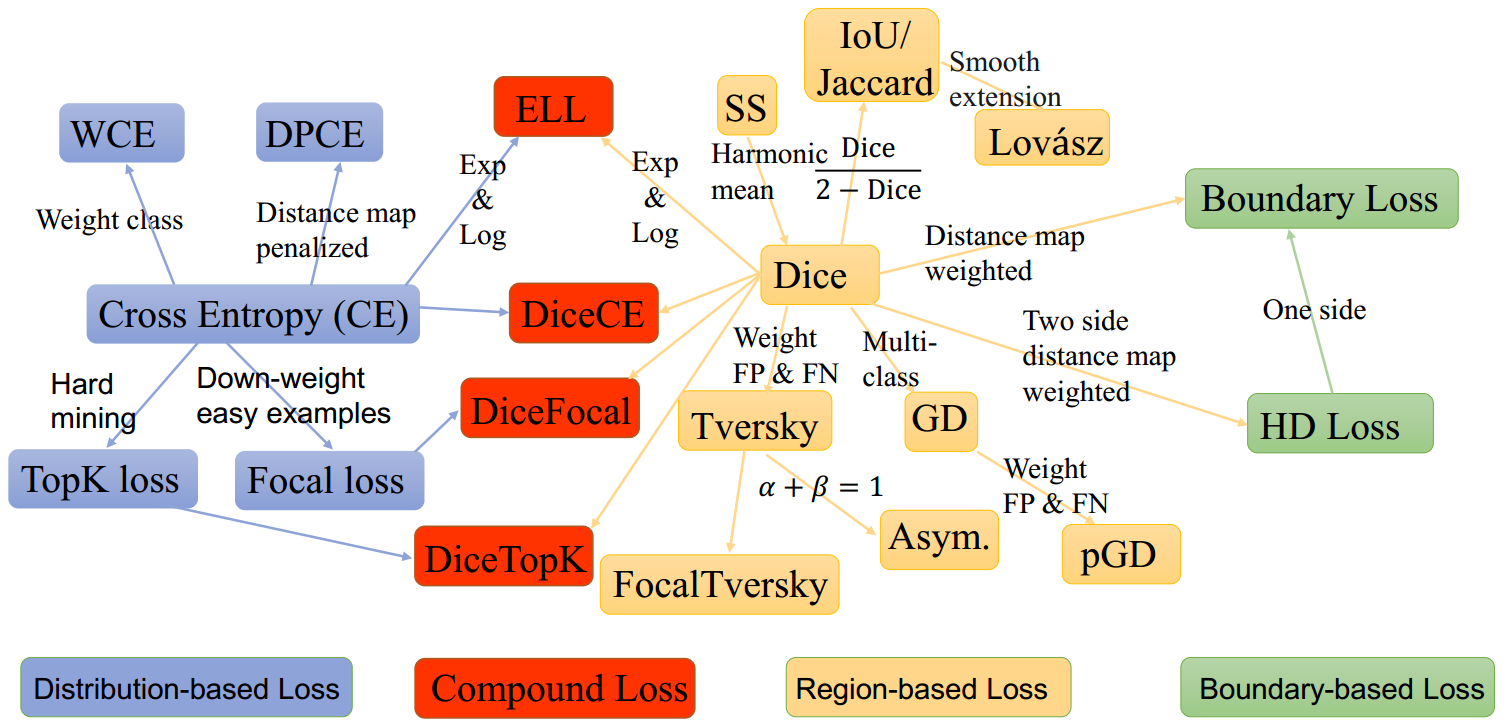
\includegraphics[width=0.75\textwidth]{LossOverview.png}
        \caption{Overview and relationship among the existing loss functions. (\cite{LossOdyssey})}
        \label{fig_loss_odissey}
    \end{figure}


\paragraph{Binary \gls{CE}}
\paragraph{}
\gls{CE} is an example of a distribution-based loss, it is derived from Kullback-Leibler (KL) divergence, which measures the dissimilarity of two distributions(\cite{LossOdyssey}). This makes the objective of this category of loss to minimise this dissimilarity. 

For this project, the most relevant \gls{CE} for binary classification tasks is the Binary \gls{CE}, which can be defined as follows:
\begin{equation} \label{eq:bintropy}
L_{B\gls{CE}} = -\frac{1}{n}\sum_{i=1}^n{[y_{i} \log(\widehat{y}_{i})+(1-y_{i})\log(1-\widehat{y}_{i})]}
\end{equation}

As in this project's data positive \gls{RTS} pixels are always underrepresented compared to background pixels, therefore the \gls{DL} network can get stuck in local minima, triggering early stopping and be very biased towards the background pixels. 
 It is relevant to mention re-weighted loss functions, where positive pixels get more importance (\cite{ronneberger2015unet}) as a potential solution.
 
Focal loss can be highlighted as a potential derivation to deal with extreme pixel class imbalance, as it reduces the relative loss of well-classified pixels by adding a factor to standard \gls{CE}, \textit{binary focal loss} is implemented as a custom loss function in section \ref{loss_exp}.
 
All the other functions depicted under the distribution-based loss in Figure \ref{fig_loss_odissey} are derivations of \gls{CE}, therefore will not be covered in detail. 
\paragraph{Dice Loss}
\paragraph{}
Dice Loss is the key element of region-based loss functions, which aim to minimise the mismatch between predicted $\widehat{y}$  and ground-truth $y$ regions (\cite{LossOdyssey}). It can directly optimise the Dice coefficient, which is defined in section \ref{performance_measures}, this was implemented as a custom loss function hereby known as \textit{dice coef loss}.

\begin{equation}\label{eq_dice_loss}
L_{dice}=1-\frac{2\sum_{{i}}^{N}\widehat{y}_{i}y_{i}}{\sum_{i}^{N}\widehat{y}_{i}^{2}+\sum_{i}^{N}y_{{i}}^{2}}
\end{equation}

\paragraph{\gls{IoU} loss}
\paragraph{}
The \gls{IoU} \gls{a.k.a.} Jaccard index is used to directly optimise the segmentation class metric, it can be seen as a similarity measure between two sets $A$ and $B$ is defined as the following:
\begin{equation}
\label{eq_jaccard}
\begin{aligned}
J(A, B) = \frac{\mid A \cap B \mid }{\mid A \cup B \mid} &= \frac{\mid A \cap B \mid}{\mid A \mid + \mid B \mid - \mid A \cap B \mid} \\ \\
0 \le & J(A, B) \le 1
\end{aligned}
\end{equation}

However, the \gls{IoU} is not differentiable, it can nonetheless be generalised for predicting probabilities, making it differentiable and therefore suitable for optimisation by gradient descent and allow for backpropagation in a \gls{NN}. This is implemented as a custom loss function and referred to later as \textit{\gls{IoU} loss}.

\begin{equation} \label{eq_iou_loss}
L_{\gls{IoU}}(y, \widehat{y}) = 1- \sum_{i=1}^n \frac{y_i \cdot \widehat{y_i}}{y_i + \widehat{y_i} - y_i \cdot \widehat{y_i}}
\end{equation}
\paragraph{}
It has been argued that \gls{IoU} loss is better for binary segmentation than those trained with the standard softmax loss(\cite{Rahman_2016}), making it a very relevant loss function for this project.
\paragraph{Compound loss}
\paragraph{}
There are many compound losses which combine and transform some loss functions introduced above. A Compound loss function, inspired by a paper (\cite{DBLP:journals/corr/IglovikovMO17}) that applies semantic segmentation to satellite imagery, appears to also be a feasible solution.
In this paper, their compound loss function is defined as a combination of Eq.\ref{eq:bintropy} and Eq.\ref{eq_iou_loss}, this will be referred to as \textit{ce jaccard loss} during implementation:
\begin{equation}
L_{\gls{CE} \gls{IoU}} = L_{B\gls{CE}} - \log (\frac{1}{n} (-L_{\gls{IoU}}+1))
\end{equation}

Another compound loss function used in this project, is a combination of Eq.\ref{eq:bintropy} and Eq.\ref{eq_dice_loss}, which will be referred to hereafter as \textit{\gls{CE} dice loss}:
\begin{equation}
L_{\gls{CE} Dice} = L_{B\gls{CE}} + L_{dice}
\end{equation}
\subsubsection{Optimiser} \label{optimiser}
\paragraph{}
In Deep Learning, optimisation refers to the process of finding the parameters $\theta$ of a \gls{NN} that attempt to minimise a loss function $J(\theta)$ (\cite{GoodBengCour16}), this process usually involves not only using usually a subset of data to calculate each update to the parameters based on an expected value of the cost function, but also taking into account any regulariser, weight initialisation, learning rate and batch size which influence the success of the optimisation strategy.

Most algorithms used for \gls{DL} use more than $1$ but less than all the training examples \gls{a.k.a.} mini-batch, even though they don't use only one example they are nowadays referred to as just stochastic methods rather than mini-batch stochastic methods. In a similarly confusing way, even though that \gls{BGD} implies the processing of the whole training set, the term batch size is usually referring to the mini-batch size, which Goodfellow et al.(\cite{GoodBengCour16}) clarifies very well.
\paragraph{\gls{SGD}}
\paragraph{}
\gls{SGD} and its variants are probably the most popular algorithms in \gls{DL} as it can converge even when the training dataset gets very large, however it has slower asymptotic convergence then \gls{BGD} for example.

\gls{SGD} aims to get an unbiased estimate of the gradient by averaging the gradient in the mini-batch drawn randomly from the training data and follow the gradient downhill (\cite{GoodBengCour16}).

The learning rate is an essential parameter in the gradient descent process, it is advised that it gradually decreases during training time, through strategies described in more detail in section \ref{learning_rate}. It is known that stochastic gradient descent has slower asymptotic convergence then \gls{BGD} for example.
\paragraph{Momentum}
\paragraph{}
Momentum has been designed to overcome \gls{SGD}'s limitations by accelerating learning, it accumulates an exponentially decaying moving average of previous gradients and keeps moving in their direction (\cite{GoodBengCour16}), creating \gls{SGD} with momentum. 

Momentum helps accelerate \gls{SGD} in the right direction and reduces oscillations (\cite{ruder2017overview}), defined by a new momentum hyperparameter $\alpha$ between $0$ and $1$, determines how quickly this moving average decays.

Common values of $\alpha$ used in practice are $0.5$, $0.9$, and $0.99$, for the semantic segmentation models introduced in section \ref{seg_nets}, the most common momentum parameter value is approximately $0.9$ (\cite{sultana2020106062})

The next few variations of stochastic gradient descent have adaptive learning rates, so it is recommended not to change the parameters in these, therefore the learning rate section \ref{learning_rate} is most relevant for the preceding optimisers.
\paragraph{\gls{RMSProp}}
\paragraph{}
\gls{RMSProp}, is an unpublished optimiser created by Tijemen Tieleman and Geoffrey Hinton in $2012$. It divides the learning rate by an exponentially decaying average of squared gradients to discard history from the extreme past so that it can converge rapi\gls{DL}y, it has been shown to be effective and practical for \gls{DL} problems (\cite{GoodBengCour16})

\paragraph{\gls{Adam}}
\paragraph{}
The \gls{Adam} optimiser (\cite{kingma2017adam}) is a variation of the combination of momentum, which points the model in a better direction and \gls{RMSProp}, which adapts how far the model goes in the direction to converge quickly.

Unlike the previous algorithms, \gls{Adam} includes bias correction to both the first-order moments (the momentum term) and the (uncentered) second-order moments (also in \gls{RMSProp}) making \gls{Adam} fairly robust to the choice of hyperparameters (\cite{GoodBengCour16}).

The authors (\cite{kingma2017adam}) show that \gls{Adam} works well in practice and compares well with other adaptive learning-method algorithms.
\paragraph{\gls{NAdam} Optimiser}
\paragraph{}
\gls{NAdam} showed dramatic improvements in this paper(\cite{nadam}) the authors argue that it is a no-brainer to incorporate Nesterov momentum into \gls{Adam}, specially where combining momentum and \gls{RMSProp} is concerned, this was actually present in Chapter 8 of Goodfellow et al.'s book (\cite{GoodBengCour16}).

It was also derived and explained by Ruder(\cite{ruder2017overview}), who also emphasizes that \gls{NAG} is superior to vanilla momentum, thus combining \gls{Adam} and NAG seems to make sense theoretically. 

Despite this claim, not many other evidences of the use of \gls{NAdam} where found in practice. Nonetheless, a technical report (\cite{DBLP:journals/corr/IglovikovMO17}) uses \gls{NAdam} as the optimiser to train a  multi-spectral image U-Net to accurately perform semantic segmentation of different classes in satellite imagery, making it quite relevant to this project.
\subsubsection{(Mini-)Batch size} \label{batch_size}
\paragraph{}
Batch size is the number of data points used to train a model in each iteration, it is very important to ensure that the algorithm converges, since it determines the frequency of updates of the network.

The larger the batch size, the more accurate cost gradient w.r.t. parameters and faster training speed (\cite{deeplearning_ai}). Large batch sizes can however negatively impact the generalisation of the network (\cite{keskar2017largebatch}).

Common mini-batch sizes range between $50$ and $256$, but vary for different applications (\cite{ruder2017overview}), for the semantic segmentation models introduced in section \ref{seg_nets} it tends to be between $12$ and $20$ images, with for example U-Net (\cite{ronneberger2015unet}) as one of the exceptions being 1 image making it a pure stochastic gradient optimisation process.
\subsubsection{Initialisation} \label{initialisation}
\paragraph{}
Some algorithms are very sensitive to weight initialisation and the success of its convergence depends a lot on the chosen initialiser. To prevent gradients from vanishing (weight initialisation too small) or exploding (too large), as a rule of thumb the mean of the activations should be $0$ and the variance of the activations should stay consistent across all layers.

For simplicity, let's assume the same initialisation methods are usually applied to both the forward propagation (activations) and backward propagation (cost gradients \gls{w.r.t.} activations).

\paragraph{Random normal initialiser} The weights are randomly initialised usually from a zero-mean normal distribution, however other values of mean and standard deviation can be defined. 

It has been used with the default configuration of zero mean and unit standard deviation in remote sensing applications by Kemker et al. (\cite{kemker2018algorithms}) in initialisation experiences Deep \gls{NN} for Semantic Segmentation.

\paragraph{Uniform initialiser} In Uniform initialisation, known to work well with the sigmoid activation function (see equation \ref{sigmoid_eq}), the weights belong to a uniform distribution in range ($a$, $b$).

\paragraph{"Xavier" (Glorot) initialiser} The "Xavier" (\cite{pmlrv9glorot10a}) initialisation, known to work well with the tanh activation function (see equation \ref{tanh_eq}), picks the weights of layer $l$ randomly from a normal distribution with mean $\mu = 0$ and variance $\sigma^2 = \frac{1}{n^{[l-1]}}$, where $n^{[l-1]}$ is the number of neurons in layer $l-1$. Biases are initialized with zeros:

$\begin{aligned}W^{[l]} &\sim \mathcal{N}(\mu=0,\sigma^2 = \frac{1}{n^{[l-1]}})\\ b^{[l]} &= 0\end{aligned}$

There is also a  "Xavier" uniform variation, where the weights are chosen from a random uniform distribution, which won't be covered in detail.
\paragraph{"He" (Kaiming) initialiser} In an attempt to discover the best initialiser to work well with \gls{ReLU} (see equation \ref{eq_relu} like activations, He et al. (\cite{He_2015_ICCV}) adapted "Xavier" initialisation to achieve better performance with rectified units, this proved quite successful as seen in Figure \ref{fig_he_xavier}.

In "He" initialisation, weights of layer $l$ are initialised with a zero-mean Gaussian distribution with a standard deviation  $\sigma =\sqrt{\frac{2}{n_l}}$, where $n_l$ is the number of activations of layer $l$. Biases are also initialized with zeros. 

The difference between this "He" and the Xavier initialisation  is the $\frac{1}{2}$ that comes from the \gls{ReLU} activation function.

\begin{figure}[hbt!]
    \centering
    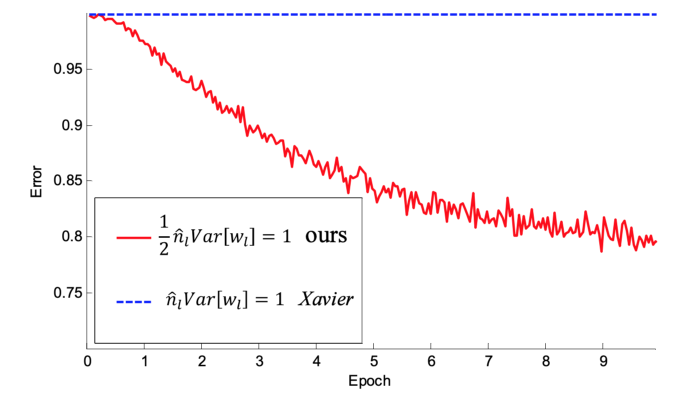
\includegraphics[width=0.5\textwidth]{xavier vs he init.png}
    \caption{Convergence of a 30-layer \gls{CNN} in He et al.'s paper (\cite{He_2015_ICCV})}
    \label{fig_he_xavier}
\end{figure}
\subsubsection{Regulariser} \label{regulariser}
When fine-tuning pre-trained models, it is very likely that overfitting will become a problem. To help address this, either $l1$  or $l2$ regularisation can be helpful with early stopping, as well as, the introduction of Dropout or Batch normalisation.
\paragraph{$l1$ and $l2$ regularisation}
Performing $l2$ regularisation \gls{a.k.a.} weight decay constrains weigh values towards 0 (but not actually zero) whereas $l1$  regularisation \gls{a.k.a.} Lasso regression drives the weights to be $0$, tends to work well as a feature selection technique. 

Regularisers are usually attached to the loss function as a penalty term, $l1$ penalises the absolute value whereas $l2$ penalises the square value of the weights (\cite{shanmugamani2018deep}). 

$l2$  is more popular, as $l1$  can remove relevant information from high-dimensional data where these are correlated, leading to underperforming models.Most of the segmentation models introduced in section \ref{seg_nets} use weight decay with values between 0.0001 and 0.0005 (\cite{sultana2020106062}).
\paragraph{Dropout} 
The idea of Dropout (\cite{JMLR:v15:srivastava14a}) is to randomly turn off neurons (along with their connections) with some probability $p$ from the \gls{NN} during training, this is usually applied at each step of forward propagation and weight update step, neurons turned off in one step can become active in the following step.

This can make this method quite computationally expensive and less effective when there are very few labelled training examples, however it does have the advantage of being (\cite{GoodBengCour16}).

In Figure \ref{fig_dropout} it can be seen that after dropout is applied in \ref{fig_dropout}b the network becomes less complex network subsampled from the original \gls{NN} in \ref{fig_dropout}a.

    \begin{figure}[hbt!]
        \centering
        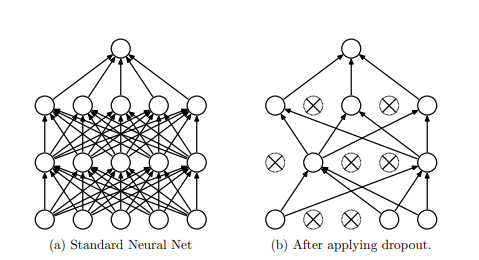
\includegraphics[width=0.6\textwidth]{droupout_example.png}
        \caption{(a) Regular 2-layer \gls{NN} (b) Example of \gls{NN} after dropout applied. Crossed neurons have been turned off. (\cite{shanmugamani2018deep})}
        \label{fig_dropout}
    \end{figure}
\paragraph{Batch Normalisation}
Its main purpose as discussed in section \ref{cnn_layers} is to make optimisation better through reparametrisation, this introduces both additive and multiplicative noise.

This noise introduced in the hidden units during training can have a regularisation effect, so that there is no need for Dropout (\cite{GoodBengCour16}).
\paragraph{Early Stopping} 
The use of early stopping is probably one of the most efficient and easy to implement regularisation methods in deep learning applications(\cite{GoodBengCour16}). It involves monitoring the parameters and validation set error, so that the best parameters at the point of the lowest validation error can be returned when the training stops. 

The training stops when none of the parameters have improved over the best validation error stored (when monitoring validation loss) for a certain number of iterations (\gls{a.k.a.} patience parameter).

It is argued that early stopping is advantageous over weight decay as it automatically figures out the correct amount of regularisation while weight decay needs several training experiments to ensure the networks doesn't get trapped in a local minimum.(\cite{GoodBengCour16}) 

\subsubsection{Learning Rate} \label{learning_rate}
\paragraph{}
Goodfellow et al. (\cite{GoodBengCour16}) suggests that the best way of choosing an initial learning rate is to monitor leaning curves, plots of loss function as a function of learning time, usually epochs. 

There are a couple of things to watch out for, big oscillations  where the loss increases drastically indicate the learning rate is too high. Small oscillations are okay, specially if the loss function contains stochastic features such as dropout. 

If the initial learning rate is too small, the function might be stuck with high loss values, getting stuck and potentially triggering early stopping. As a rule of thumb, it is advised that the initial learning rate is higher than the best performing rate after approximately $100$ iterations(\cite{GoodBengCour16}).
\paragraph{Linear Decay} 
It is common to decay the learning rate until it makes a couple of hundred passes through the training dataset (until iteration $\tau$)(\cite{GoodBengCour16}). Therefore, we define learning rate at iteration $k$ as $\epsilon_k$:

\begin{equation} \label{eq_linear_lr}
\epsilon_k = (1 - \alpha)\epsilon_0 + \alpha\epsilon_\tau
\end{equation}
where $\alpha=\frac{k}{\tau}$. After iteration $\tau$ , it is usual to leave $\epsilon$ constant.
\paragraph{Step Decay} 
Step decay drops the learning rate by a factor every few epochs. For example, in the DeepLab model's original paper (\cite{chen2016semantic}) uses a $\epsilon_0=0.001$ and an $\epsilon_\tau=0.01$ in the final classification layer. It drops it $10\%$ by multiplying it by $0.1$ at every $2000$ iterations.
\paragraph{Exponential Decay} 
As the name implies, an exponential decay function is applied to the initial learning rate $\epsilon_0$:

\begin{equation} \label{eq_exp_lr}
\epsilon_k = \epsilon_0e^{-\alpha k}
\end{equation} 
where $\alpha$ is the exponential decay parameter.

For example, in a paper that introduces the \gls{FCN}-DenseNer103(\cite{Jegou_2017_CVPR_Workshops}) the authors use $\epsilon_0=0.001$ with an exponential decay of $0.995$ every epoch.
\paragraph{Polynomial decay policy ("poly")} 

Starting with ParseNet (\cite{liu2015parsenet}), where the authors improved the performance of their model by $1.5\%$ with the same iterations (80k), $\epsilon_0= 1e^-9 $ and  $power=0.9$, it is proved to converge faster than step decay. 

ParseNet inspired the authors of Deeplab model's follow-up paper in 2017 (\cite{chen2017deeplab}) to also use “poly” ($power=0.9$), using the same batch size and training iterations they also achieve better performance ($1.17\%$)than "step", reinforcing the trend. 

The creators of the Pyramid Parsing Network (PSPNet) (\cite{zhao2017pyramid}), another popular semantic segmentation model, yet again inspired by DeepLab, also use ‘poly’ learning rate with $\epsilon_0= 0.01$ and $power=0.9$. This popular learning rate policy among state-of-the-art semantic segmentation model is defined in Equation \ref{eq_poly_lr} below:

\begin{equation} \label{eq_poly_lr}
\epsilon_k=\epsilon_0(1- \frac{k}{T_{k}})^{power} 
\end{equation}

where $T_{k}$ is the total number of iterations and $power$ term controls the shape of the learning rate decay. In case of polynomial learning rate policy, $T_{k}$ is equal to total number of epochs times number of iterations in an epoch (\cite{8929465}).

There are many other learning rate policies such as the constant learning rate, manual step learning rate and cosine decay learning rate that are self-explanatory, so will not be covered in detail.
\subsection{Measurement of model performance} \label{performance_measures}
\paragraph{}
During training, it is usual to monitor certain metrics that measure how well the model is performing, ones typically used in semantic segmentation problems are outlined in this section.
\paragraph{Dice coefficient}
The dice coefficient (\cite{7785132}), ranging between $0$ and $1$, is the most commonly used segmentation evaluation metric. The Dice coefficient ($Dice$) between $2$ binary volumes, which the aim is to maximise, can be written as:

\begin{equation}
    \label{eq_dice_coef}
    Dice=\frac{2\sum_{{i}}^{N}p_{i}g_{i}}{\sum_{i}^{N}p_{i}^{2}+\sum_{i}^{N}g_{{i}}^{2}}
\end{equation}

\paragraph{\gls{IoU}}
From the definition of the two metrics, we have that \gls{IoU} and Dice score are within a factor of $2$ of each other $F/2 \leq \gls{IoU} \leq F$. It has been defined in section \ref{loss_functions} with Equation \ref{eq_jaccard}

In general, like $l2$ penalises the biggest mistakes more than $l1$ regularisation, the \gls{IoU} metric penalises a single instances of wrong classification more than the Dice score. The \gls{IoU} metric has a "squaring" effect on the errors in comparison with the Dice score, making it more focused on the worst performance, rather than the average.

\subsection{Transfer Learning} \label{transfer_learning}
\paragraph{}
Due to the small training set, it is advisable to use pre-trained weights on other datasets to accelerate the training process, this is known as transfer learning and it as become a widely used technique in accelerating progress in the field of \gls{CV}.

It is the process of initialising a model using the weights of another model pre-trained on a much larger dataset, this usually ensures faster convergence. (\cite{shanmugamani2018deep})

As a rule of thumb, one can either use the pre-trained model as is, or pick and choose which layers to re-train or fine-tune depending on the problem at hand as outlined in table \ref{table_transfer_learn}.

\begin{center}
    \begin{tabular}{c|c|c}     \label{table_transfer_learn}
    \textbf{Sample size} & \textbf{Dataset Similarity} & \textbf{Dataset Difference} \\
    \hline
    Small Data 
    &  Fine-tune output layers
    & Fine-tune hidden layers  \\
    \hline
    Big Data 
    &  Fine-tune whole model
    & Re-train model  \\
    \end{tabular}
\end{center}
